\documentclass{article}
             \usepackage{graphicx}
             \usepackage[colorlinks]{hyperref} 
             \usepackage{url}
             \usepackage{float}
             \usepackage[landscape]{geometry} 
\title{Report generated by Pmetrics package for R on 27 Jul 2015 at 06:33 } 
\date{}
              \begin{document}
              \maketitle 
Laboratory of Applied Pharmacokinetics $\cdot$ 4650 Sunset Blvd. MS\#51, Los Angeles, CA 90027 $\cdot$ (323) 361-5046 $\cdot$ \href{http://www.lapk.org}{www.lapk.org} 
\hypertarget{tableofcontents}{}
        \tableofcontents
        \newpage 
\section{Summary} \hyperlink{tableofcontents}{Back to Contents} $\cdot$ \hyperlink{cycleinfo}{Next Section}\newline
 \newline 
Engine: NPAG\newline 
Output file: /Users/Neely/LAPK/PmetricsSource/Test/NPAG/5/outputs/NP\_RF0001.TXT\newline 
Random parameters:Ka, Ke, V, Tlag1\newline 
There were no fixed parameters. \newline 
Number of analyzed subjects:  20 \newline 
Number of output equations:  1 \newline 
Number of cycles:  100     *The run did not converge before the last cycle. \newline 
Additional covariates:  WT, AFRICA, AGE, GENDER, HEIGHT \newline 
Prior density: Uniform \newline Assay error model: SD, gamma \newline  \newline 
\newpage
            \hypertarget{cycleinfo}{}
            
            \section{Cycle information} \  
 $\cdot$ \hyperlink{tableofcontents}{Back to Contents} $\cdot$ \hyperlink{mppd}{Next Section} \newline 
\begin{figure}[H] 
            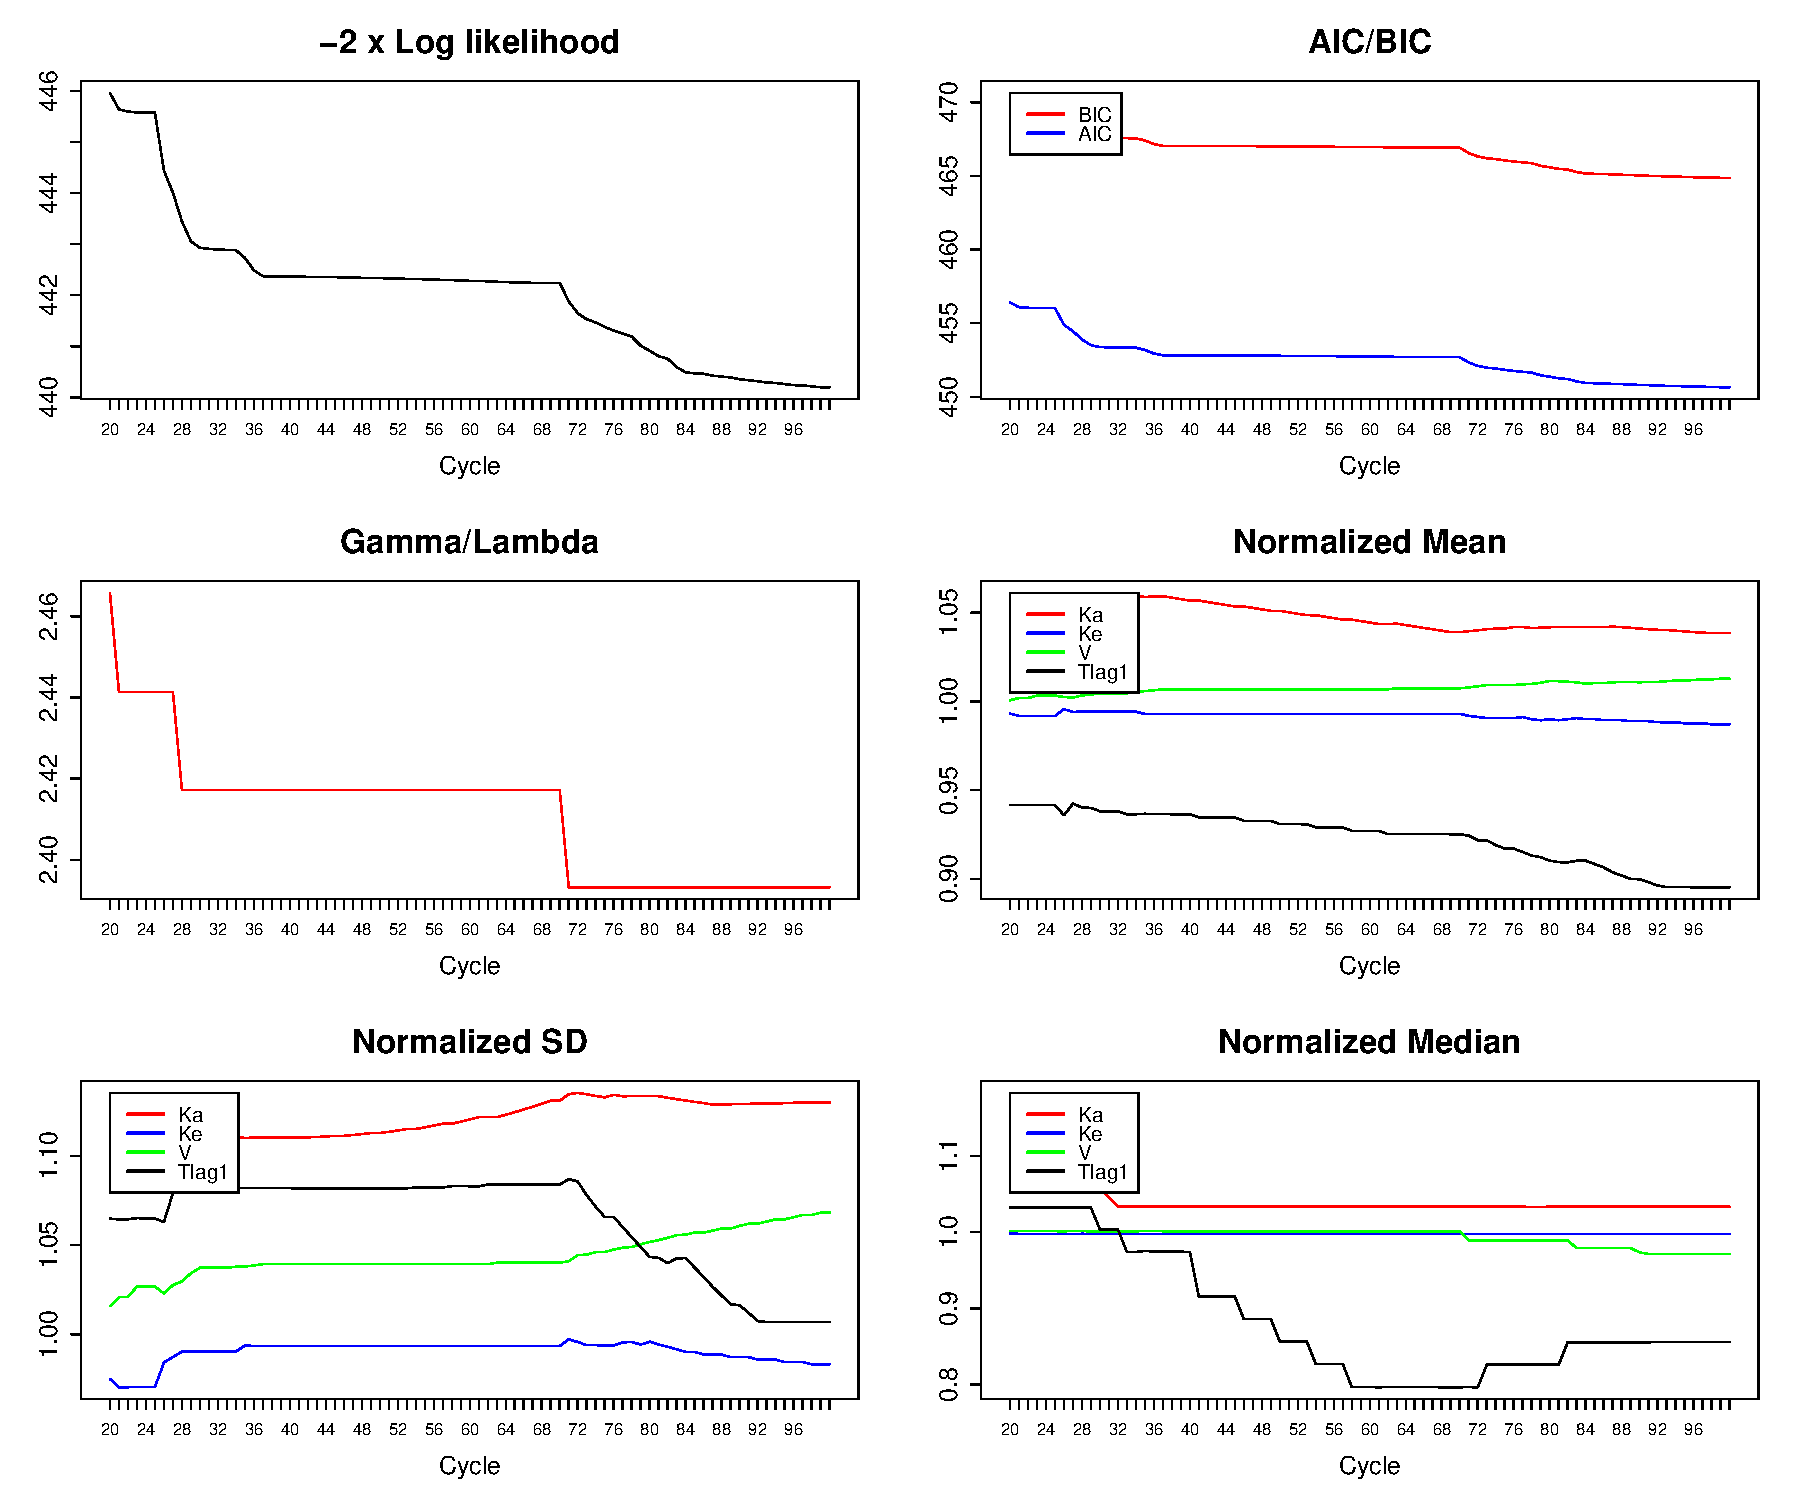
\includegraphics[height=4.99in,width=7in]{cycle.pdf}
            \end{figure} 
\hypertarget{mppd}{}
          \section{Marginal population parameter distributions} 
 $\cdot$ \hyperlink{tableofcontents}{Back to Contents} $\cdot$ \hyperlink{suppoint}{Next Section} \newline
           
\begin{figure}[H] 
          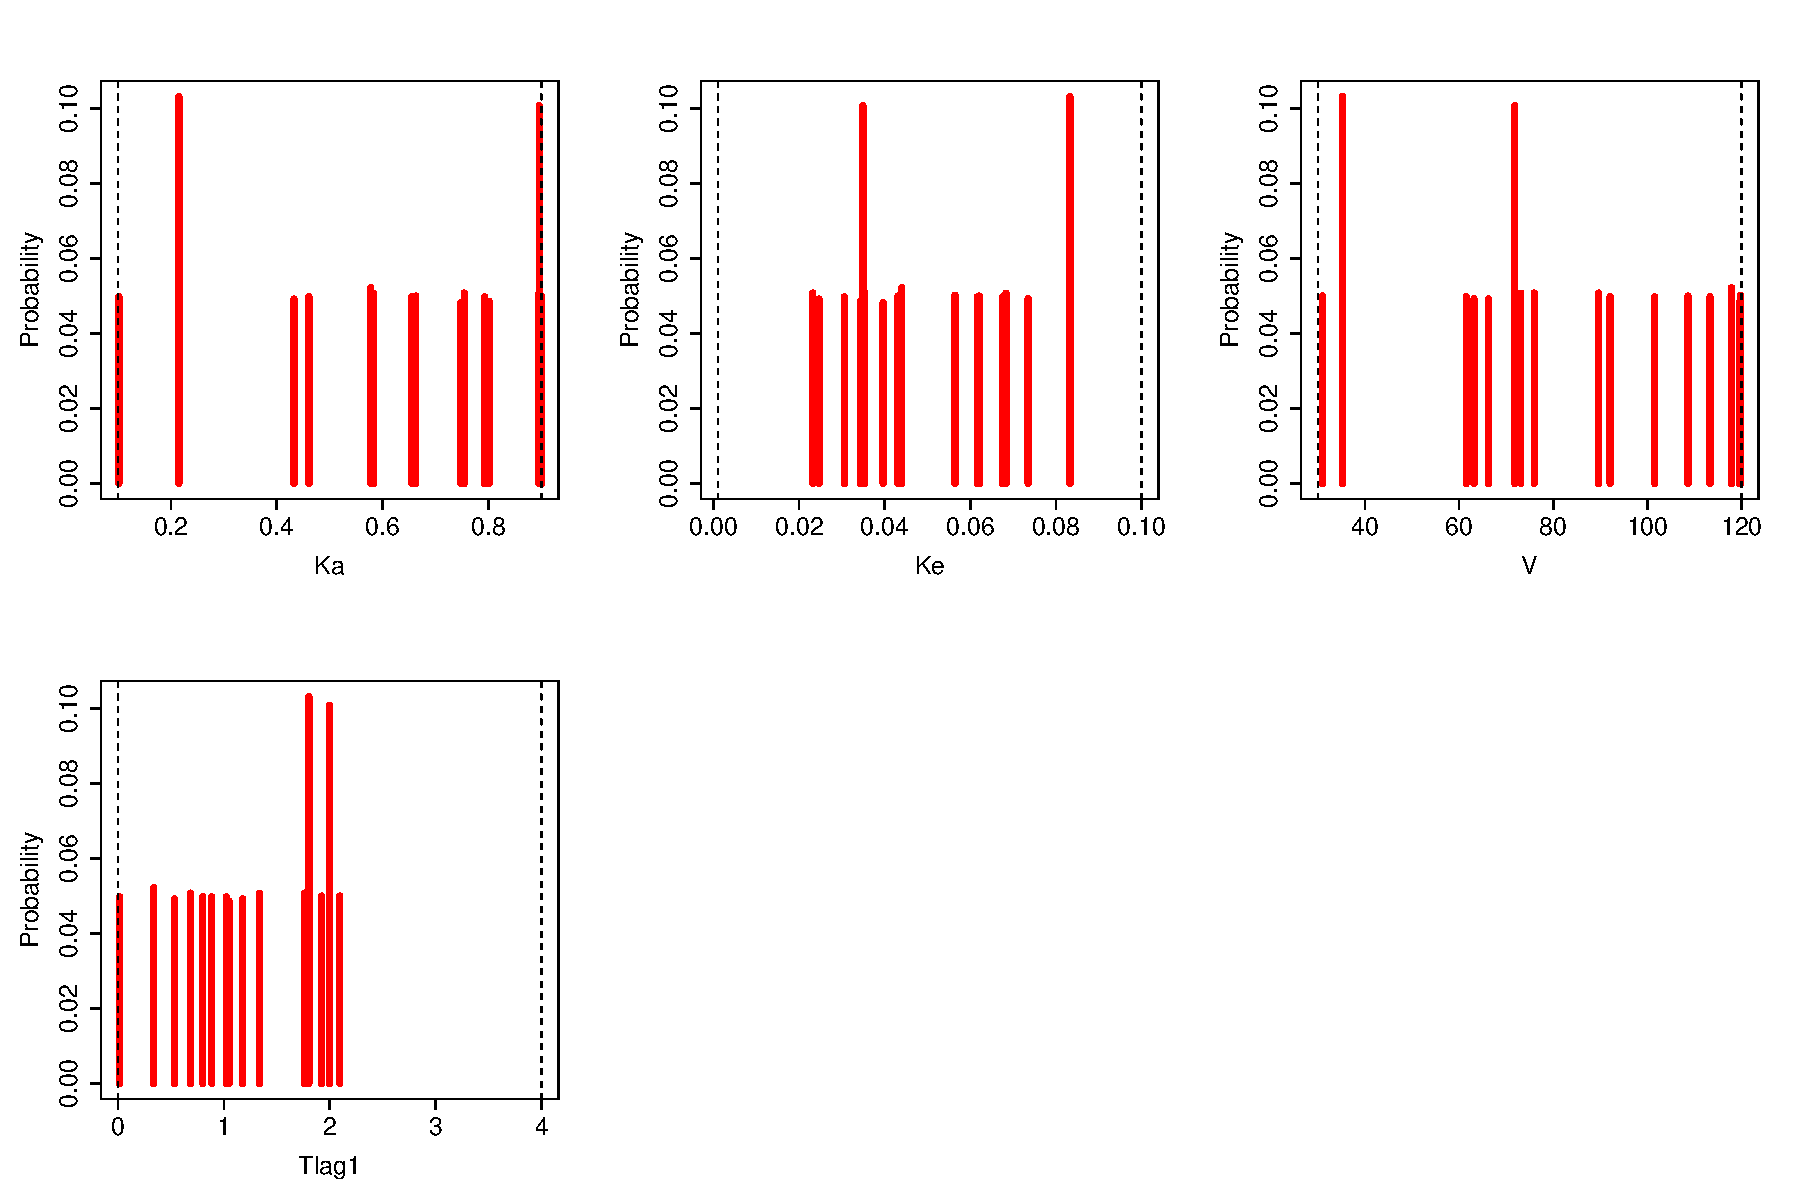
\includegraphics[height=4.5in,width=8in]{final.pdf}
          \end{figure} 
              
          \hypertarget{suppoint}{}
          
          \section{Support points} 
 $\cdot$ \hyperlink{tableofcontents}{Back to Contents} $\cdot$ \hyperlink{ppe}{Next Section} \newline
          \newline 
% latex table generated in R 3.2.1 by xtable 1.7-4 package
% Mon Jul 27 06:33:33 2015
\begin{tabular}{rrrrrr}
  \hline
 & Ka & Ke & V & Tlag1 & prob \\ 
  \hline
1 & 0.66 & 0.06 & 30.98 & 1.92 & 0.05 \\ 
  2 & 0.90 & 0.04 & 108.65 & 2.10 & 0.05 \\ 
  3 & 0.22 & 0.08 & 35.22 & 1.80 & 0.10 \\ 
  4 & 0.79 & 0.04 & 101.57 & 0.89 & 0.05 \\ 
  5 & 0.58 & 0.04 & 117.88 & 0.34 & 0.05 \\ 
  6 & 0.66 & 0.06 & 61.52 & 0.80 & 0.05 \\ 
  7 & 0.75 & 0.04 & 89.66 & 0.69 & 0.05 \\ 
  8 & 0.90 & 0.02 & 75.94 & 1.76 & 0.05 \\ 
  9 & 0.22 & 0.08 & 35.22 & 1.78 & 0.05 \\ 
  10 & 0.43 & 0.02 & 66.23 & 0.53 & 0.05 \\ 
  11 & 0.90 & 0.06 & 119.82 & 0.69 & 0.05 \\ 
  12 & 0.80 & 0.03 & 71.83 & 1.05 & 0.05 \\ 
  13 & 0.75 & 0.04 & 119.57 & 0.01 & 0.05 \\ 
  14 & 0.90 & 0.07 & 63.16 & 1.18 & 0.05 \\ 
  15 & 0.46 & 0.03 & 92.08 & 1.02 & 0.05 \\ 
  16 & 0.90 & 0.03 & 71.83 & 2.00 & 0.10 \\ 
  17 & 0.58 & 0.07 & 73.12 & 1.34 & 0.05 \\ 
  18 & 0.10 & 0.07 & 113.32 & 0.02 & 0.05 \\ 
   \hline
\end{tabular}
              
          \hypertarget{ppe}{}
          
          \section{Population parameter estimate summary statistics} 
 \hyperlink{tableofcontents}{Back to Contents} $\cdot$ \hyperlink{covforppe}{Next Section} \newline
          \newline 
% latex table generated in R 3.2.1 by xtable 1.7-4 package
% Mon Jul 27 06:33:33 2015
\begin{tabular}{rrrrrr}
  \hline
 & mean & sd & CV & var & median \\ 
  \hline
Ka & 0.63 & 0.26 & 41.71 & 0.07 & 0.71 \\ 
  Ke & 0.05 & 0.02 & 38.15 & 0.00 & 0.04 \\ 
  V & 77.77 & 28.83 & 37.06 & 830.92 & 72.48 \\ 
  Tlag1 & 1.19 & 0.66 & 55.93 & 0.44 & 1.11 \\ 
   \hline
\end{tabular}
\newpage
          
          \hypertarget{covforppe}{}
          
          \section{Covariance matrix for population parameter estimates} 
 \hyperlink{tableofcontents}{Back to Contents} $\cdot$ \hyperlink{corforppe}{Next Section} \newline
          \newline 
% latex table generated in R 3.2.1 by xtable 1.7-4 package
% Mon Jul 27 06:33:33 2015
\begin{tabular}{rrrrr}
  \hline
 & Ka & Ke & V & Tlag1 \\ 
  \hline
Ka & 0.07 & -0.00 & 2.57 & 0.02 \\ 
  Ke & -0.00 & 0.00 & -0.27 & 0.00 \\ 
  V & 2.57 & -0.27 & 830.92 & -12.10 \\ 
  Tlag1 & 0.02 & 0.00 & -12.10 & 0.44 \\ 
   \hline
\end{tabular}

          \hypertarget{corforppe}{}
          
          \section{Correlation matrix for population parameter estimates} 
 \hyperlink{tableofcontents}{Back to Contents} $\cdot$ \hyperlink{opp}{Next Section} \newline
          \newline 
% latex table generated in R 3.2.1 by xtable 1.7-4 package
% Mon Jul 27 06:33:33 2015
\begin{tabular}{rrrrr}
  \hline
 & Ka & Ke & V & Tlag1 \\ 
  \hline
Ka & 1.00 & -0.57 & 0.34 & 0.14 \\ 
  Ke & -0.57 & 1.00 & -0.48 & 0.17 \\ 
  V & 0.34 & -0.48 & 1.00 & -0.63 \\ 
  Tlag1 & 0.14 & 0.17 & -0.63 & 1.00 \\ 
   \hline
\end{tabular}
\newpage
        
        \hypertarget{opp}{}
        
        \section{Observed vs. predicted plots}
        \hyperlink{tableofcontents}{Back to Contents} \newline
        \newline 
Output 1 
\begin{figure}[H] 
              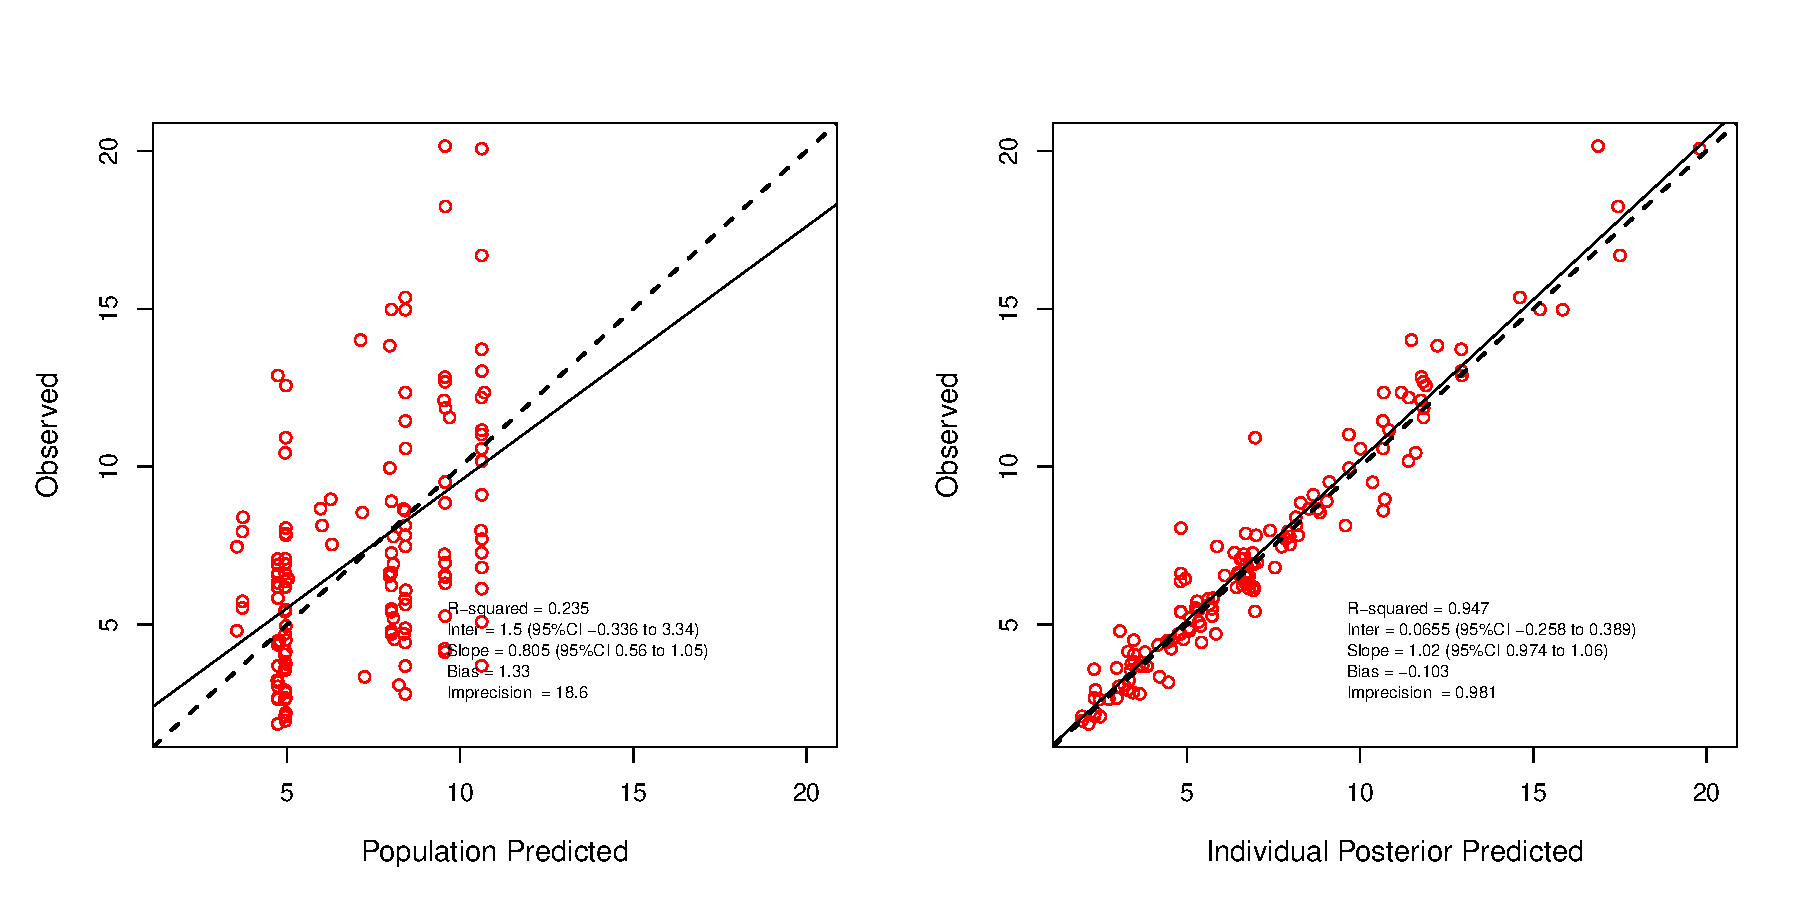
\includegraphics[height=4.5in,width=8in]{op1.pdf} 
              \end{figure} 
\end{document} 
